\chapter{Otro capítulo}

\section{Esta es una sección}

\begin{itemize}
    \item Cursiva \textit{así}
    \item Negrita \textbf{así}
    \item ``Enfatizar" \emph{así}
    \item <<Inclinada>> \textsl{así}
    \item Versalitas \textsc{Así}
\end{itemize}

\begin{enumerate}
    \item Opción 1
    \item Opción 2
    \item Opción 3
\end{enumerate}

\subsection{Entornos}

Ahora mostraremos cómo quedan algunos entornos:

\begin{enumerate}
   \item Primera opción primer nivel
   \item Segunda opción primer nivel
   \begin{enumerate}
     \item Primera opción segundo nivel
     \item Segunda opción segundo nivel
     \begin{enumerate}
       \item Primera opción nivel tres
       \item Segunda opción nivel tres
     \end{enumerate}
   \end{enumerate}
 \end{enumerate}
 
\begin{figure}[htp]
	\centering
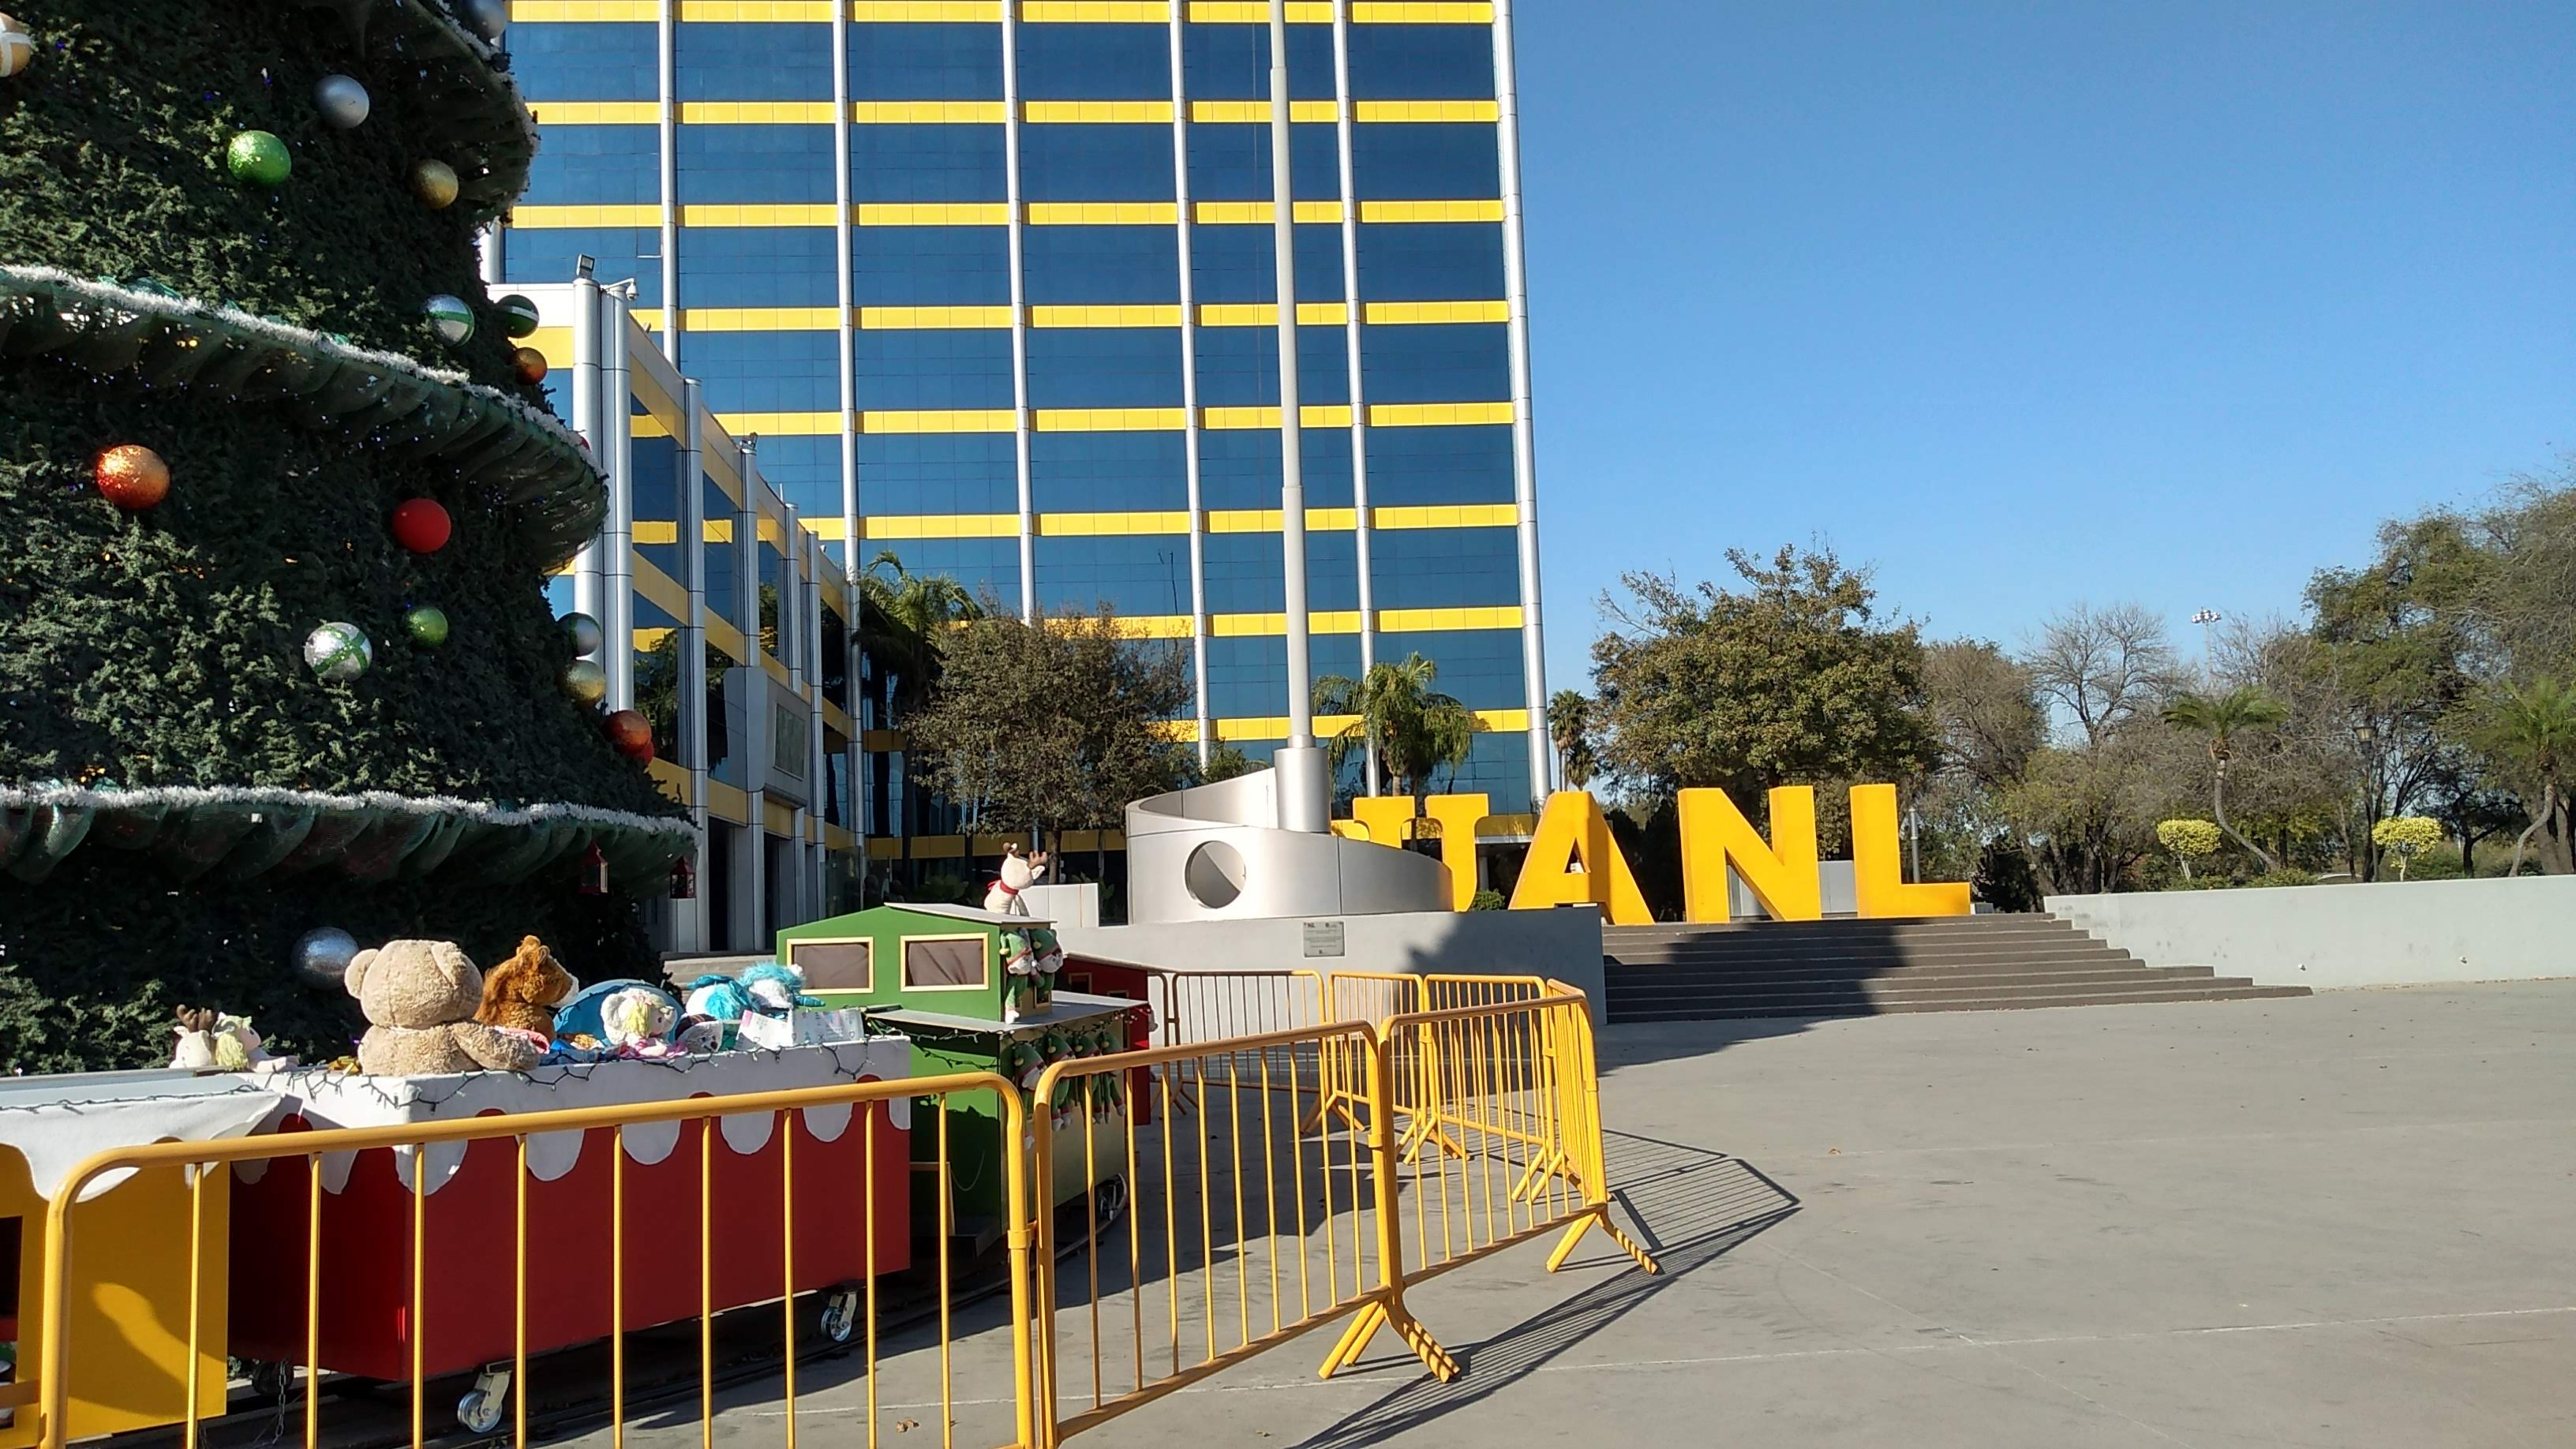
\includegraphics[width=8cm]{Figuras/Invierno UANL.jpg}
	\caption[Edificio de Rectoría]{El edificio de Rectoría de la UANL}
	\label{fig:uanl}
\end{figure}